\documentclass{article}
\usepackage{physics}
\usepackage{graphicx}
\usepackage{caption}
\usepackage{amsmath}
\usepackage{bm}
\usepackage{framed}
\usepackage{authblk}
\usepackage{empheq}
\usepackage{amsfonts}
\usepackage{esint}
\usepackage[makeroom]{cancel}
\usepackage{dsfont}
\usepackage{centernot}
\usepackage{mathtools}
\usepackage{bigints}
\usepackage{amsthm}
\theoremstyle{definition}
\newtheorem{defn}{Definition}[section]
\newtheorem{prop}{Proposition}[section]
\newtheorem{rmk}{Remark}[section]
\newtheorem{thm}{Theorem}[section]
\newtheorem{exmp}{Example}[section]
\newtheorem{prob}{Problem}[section]
\newtheorem{sln}{Solution}[section]
\newtheorem*{prob*}{Problem}
\newtheorem{exer}{Exercise}[section]
\newtheorem*{exer*}{Exercise}
\newtheorem*{sln*}{Solution}
\usepackage{empheq}
\usepackage{tensor}
\usepackage{xcolor}
%\definecolor{colby}{rgb}{0.0, 0.0, 0.5}
\definecolor{MIT}{RGB}{163, 31, 52}
\usepackage[pdftex]{hyperref}
%\hypersetup{colorlinks,urlcolor=colby}
\hypersetup{colorlinks,linkcolor={MIT},citecolor={MIT},urlcolor={MIT}}  



\newcommand*\widefbox[1]{\fbox{\hspace{2em}#1\hspace{2em}}}

\newcommand{\p}{\partial}
\newcommand{\R}{\mathbb{R}}
\newcommand{\C}{\mathbb{C}}
\newcommand{\lag}{\mathcal{L}}
\newcommand{\nn}{\nonumber}
\newcommand{\ham}{\mathcal{H}}
\newcommand{\M}{\mathcal{M}}
\newcommand{\I}{\mathcal{I}}
\newcommand{\K}{\mathcal{K}}
\newcommand{\F}{\mathcal{F}}
\newcommand{\w}{\omega}
\newcommand{\lam}{\lambda}
\newcommand{\al}{\alpha}
\newcommand{\be}{\beta}
\newcommand{\x}{\xi}

\newcommand{\G}{\mathcal{G}}

\newcommand{\f}[2]{\frac{#1}{#2}}

\newcommand{\ift}{\infty}

\newcommand{\lp}{\left(}
\newcommand{\rp}{\right)}

\newcommand{\lb}{\left[}
\newcommand{\rb}{\right]}

\newcommand{\lc}{\left\{}
\newcommand{\rc}{\right\}}


\newcommand{\V}{\mathbf{V}}
\newcommand{\U}{\mathcal{U}}
\newcommand{\Id}{\mathcal{I}}
\newcommand{\D}{\mathcal{D}}
\newcommand{\Z}{\mathcal{Z}}

%\setcounter{chapter}{-1}






\usepackage{subfig}
\usepackage{listings}
\captionsetup[lstlisting]{margin=0cm,format=hang,font=small,format=plain,labelfont={bf,up},textfont={it}}
\renewcommand*{\lstlistingname}{Code \textcolor{violet}{\textsl{Mathematica}}}
\definecolor{gris245}{RGB}{245,245,245}
\definecolor{olive}{RGB}{50,140,50}
\definecolor{brun}{RGB}{175,100,80}

%\hypersetup{colorlinks,urlcolor=colby}
\lstset{
	tabsize=4,
	frame=single,
	language=mathematica,
	basicstyle=\scriptsize\ttfamily,
	keywordstyle=\color{black},
	backgroundcolor=\color{gris245},
	commentstyle=\color{gray},
	showstringspaces=false,
	emph={
		r1,
		r2,
		epsilon,epsilon_,
		Newton,Newton_
	},emphstyle={\color{olive}},
	emph={[2]
		L,
		CouleurCourbe,
		PotentielEffectif,
		IdCourbe,
		Courbe
	},emphstyle={[2]\color{blue}},
	emph={[3]r,r_,n,n_},emphstyle={[3]\color{magenta}}
}


\begin{document}

\title{A quick guide to PID Feedback Control}
\author{HUAN Q. BUI}	
\maketitle



\section{An Example and Theory}

Consider a 1D harmonic oscillator with natural resonance frequency $\omega_0$ and damping parameter $\beta$, driven by some function $y(t)$. Its motion follows the following second-order ordinary differential equation:
\begin{equation*}
\ddot{x}(t) + \be \dot{x}(t) + \omega_0^2 x(t) = \omega_0^2 y(t).
\end{equation*}

There are many ways to solve this ODE, but in the context of control theory, we will proceed using the Fourier transform (or the Laplace transform). The point of the FT is twofold: (1) we convert a differential equation into an algebraic equation, and (2) we from the time domain to the frequency domain, where analysis becomes more ``intuitive'' (eventually, anyway). \\

In any case, define the FT of $x(t)$ as 
\begin{equation*}
x(\omega) = \int \f{d t }{2\pi } e^{i\omega t} x(t). 
\end{equation*}
We note that factors of $2\pi$ don't really matter here since we now take the FT of both sides of the ODE to find
\begin{equation}\label{eq:ODE}
-\omega^2 x(\omega) + i\beta \omega x(\omega) + \omega_0^2 x(\omega) = \omega_0^2 y(\omega).
\end{equation}
Here, we have used the following identity:
\begin{equation*}
\F\lb \f{d^n }{dt^n} x(t) \rb = (i\omega)^n x(\omega).
\end{equation*}
From \eqref{eq:ODE}, we can define $G(\omega)$, the \textbf{impulse response function} (in frequency domain) as the ratio of output $x(\omega)$ over input $y(\omega)$:
\begin{equation*}
G(\omega) \equiv \f{x(\omega)}{y(\omega)} = \f{1}{(\omega_0^2 - \omega^2) + i\beta \omega}
\end{equation*}
We can justify why $G$ is called as such by considering the impulse input $y(t) = y_0 \delta(t)$ and find that $G(\omega) = x(\omega)/y_0$. More commonly, $G(\omega)$ is also known as the \textbf{transfer function} of the system.\footnote{There might be some confusion here regarding whether to use the Fourier or Laplace transform. Here's the resolution: If we're using the FT, then evaluate $G$ at $\omega\in \mathbb{R}$. If we're using the LT, then evaluate $G$ at $i\omega$.}\\


We have basically solved the problem: given some input $y(\omega)$, we can inverse-FT to find $x(t)$ from $x(\omega)$ via $G(\omega)$. Now, suppose we want to control the position of the oscillator so that $x(t)$ follows some desired position $r(t)$ as faithfully as possible. How do we do this? \\


A first guess is setting the driving function to be the desired position, i.e., $y(t) = r(t)$. In this case, we have 
\begin{equation*}
x(\omega) = G(\omega) r(\omega).
\end{equation*}
A convenient way to see how the system may respond to any driving function is to study the transfer function $G(\omega)$ using the \textbf{amplitude} and \textbf{phase Bode plots}. The former is almost always a log-log plot, while the latter can either be a linear-linear or log-linear plot. For our system, we can generate these plots (Figure \ref{fig:bode_1}) in Mathematica using the following code. 

\begin{lstlisting}
\[Beta] = 2; \[Omega]0 = 2*Pi;

G[\[Omega]_] := \[Omega]0^2/((\[Omega]0^2 - \[Omega]^2) + 
I*\[Beta]*\[Omega]);

LogLogPlot[Abs[G[a*\[Omega]0]], {a, 0, 10}, PlotRange -> Full, 
AxesLabel -> {\[Omega]/"\[Omega]0", Abs[G]}]

LogLinearPlot[Arg[G[a*\[Omega]0]], {a, 0.01, 200}, 
AxesLabel -> {\[Omega]/"\[Omega]0", Arg[G]}]
\end{lstlisting}


\begin{figure}
	\centering
	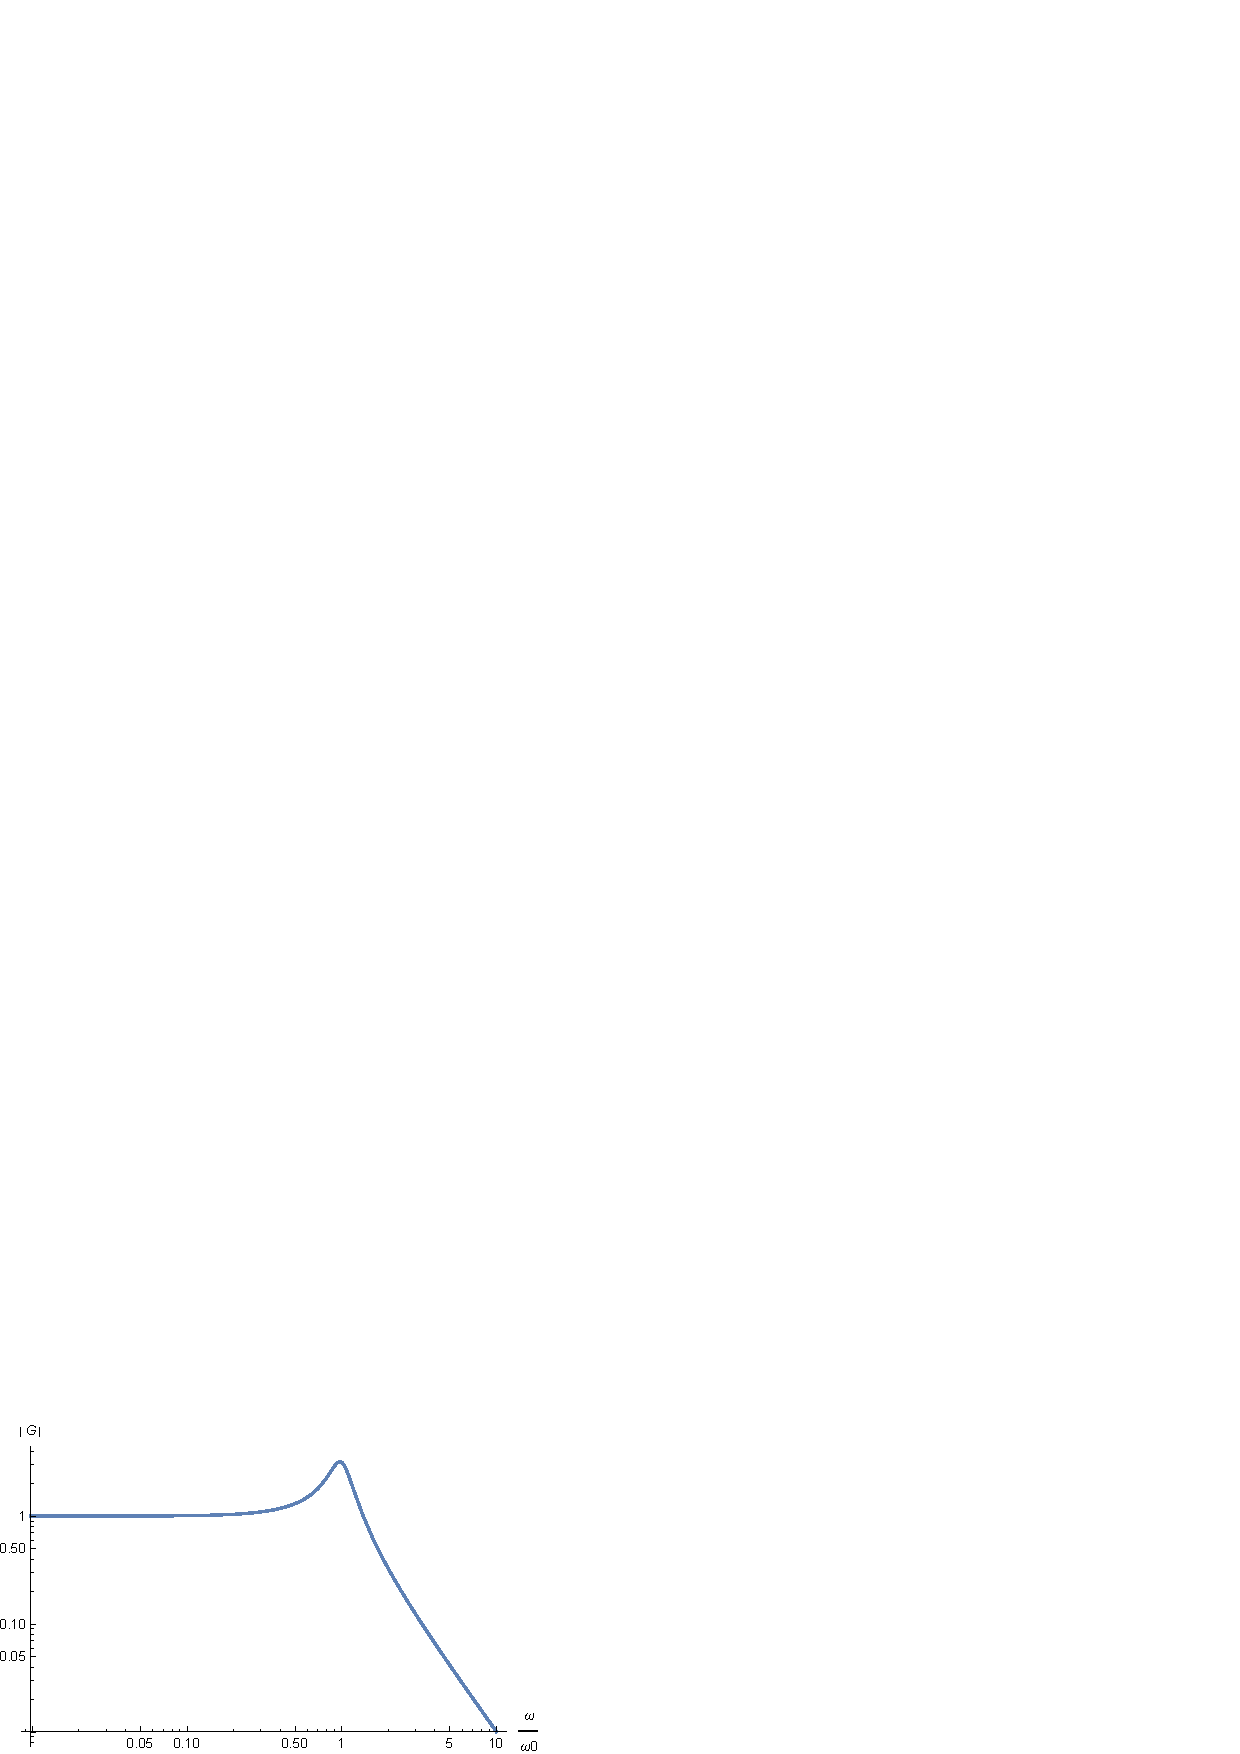
\includegraphics[width=0.45\textwidth]{bode_1}
	\quad
	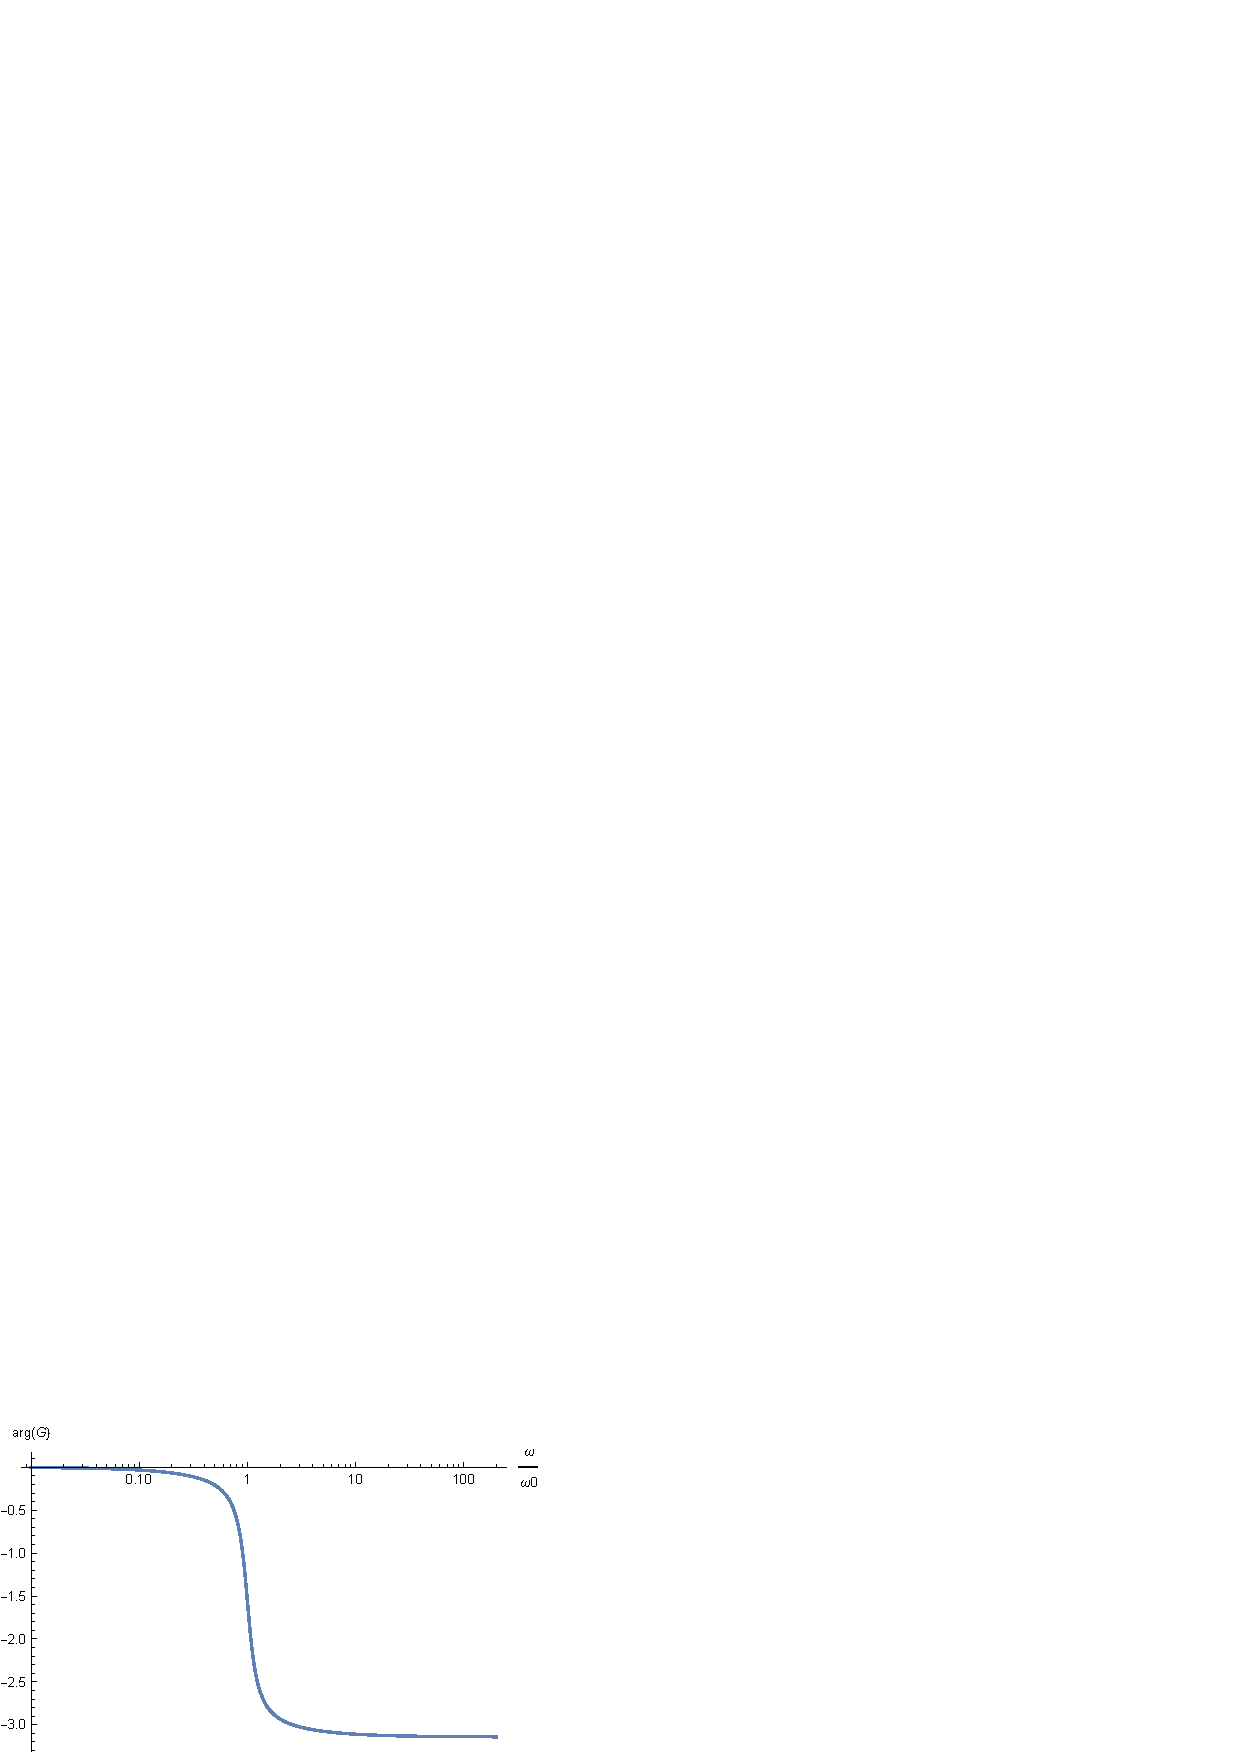
\includegraphics[width=0.45\textwidth]{bode_2}
	\caption{Bode plots for the transfer function $G$ with $\beta = 2,\omega_0 = 2\pi$. The plot on the left is the amplitude Bode plot; the plot on the right shows the phase. Notice how $\abs{G}$ exceeds \textbf{unity} when $\omega \approx \omega_0$ (resonance!). Notice also on the phase Bode plot how the phase lags behind as $\omega$ grows and exceeds $\omega_0$.}%
	\label{fig:bode_1}
\end{figure}



To continue our analysis, we consider different regimes for $\omega$:
\begin{itemize}
	\item  For low frequencies ($\omega \ll \omega_0$), the system follows the drive quite well: $\abs{G} \approx 1$ and the phase lag $\arg(G) \approx 0$.
	
	\item However, as we approach the resonance frequency $\omega_0$ we become ``too slow'' because both $\abs{G}$ and $\arg(G)$ deviate from ``unity,'' and $x(\omega)$ no longer follows $r(\omega)$ well.
	
	
	\item  On resonance ($\omega = \omega_0$), the amplitude becomes larger than that of the reference: 
	\begin{equation*}
	\abs{x(\omega_0)} = \abs{G(\omega_0)}\abs{r(\omega_0)} = \f{\omega_0}{\beta} \abs{r(\omega_0)} = Q\abs{r(\omega_0)}, 
	\end{equation*}
	where $Q$ is the \textbf{quality factor} of the oscillator. Meanwhile, the phase lags behind by 
	\begin{equation*}
	\arg(G(\omega_0)) = \arg\lp -i\f{\omega_0}{\beta} \rp = \f{\pi}{2}.
	\end{equation*}
	
	
	\item For higher frequencies, we can take some limits and find that the phase lags by $\pi$ and the amplitude decreases like 
	\begin{equation*}
	\abs{x(\omega)} \to \f{\omega_0^2}{\omega^2}\abs{r(\omega)}.
	\end{equation*}
	Because of this, we see a drop in frequency response in the amplitude Bode plot when $\omega \gg \omega_0$. The asymptote here is $\omega_0^2/\omega^2$, which appears on the log scale as a straight line. 
\end{itemize}




So, we have a problem: using $y(t) = r(t)$ itself as a driving function is only good when $\omega$ is very small. But there's a way around this (otherwise this article wouldn't exist). For our system to follow $r(t)$ more faithfully, the driving function must also take into account the current position $x(t)$ \textbf{relative} to the reference $r(t)$. This is \textbf{feedback}: we control our system based on not just the reference but also the current state of the system. Feedback is nice because it detects if the system lags behind or if its amplitude is too large or too small and tries to compensate accordingly. Furthermore, it allows us to correct for \textbf{noise}, which appears in all real system. While we can simply let some function $\xi(t)$ represent noise, we won't worry about it for the forthcoming part of our analysis. \\


What we have to do now is instead of naively setting $y(t) = r(t)$, we will first define some \textbf{error signal} $\epsilon(t)$ and try to minimize it. The error signal is simply how far away our system is from the reference:
\begin{equation*}
\epsilon(t) = r(t) - x(t).
\end{equation*}

With the error signal, we can now define the driving function $y(t)$ such that $y(t)$ changes the system to minimize $e(t)$. This is where the three letters \textbf{P-I-D} come in. Intuitively, we want $y(t)$ to do the following things:
\begin{itemize}
	\item If $\epsilon(t)$ is large (large error), then $y(t)$ should also be large (large correction), and vice versa. So, we can set $y(t) = K_p \epsilon(t)$. This is \textbf{P}, which stands for \textbf{Proportional}. Here $K_p$ is called the \textbf{proportional gain}. 
	
	
	\item If $\epsilon(t)$ has been large \textit{so far} (still far away from reference), then $y(t)$ must also be large (move faster towards reference), and vice versa. We can set $y(t) = K_i \int_0^t \epsilon(t')\,dt'$. This is \textbf{I}, which stands for \textbf{Integral}. Here, $K_i$ is called the \textbf{integral gain}. \footnote{The lower bound of the integral can be $0$ or $-\infty$ -- this doesn't really matter too much here.}
	
	
	\item If $\epsilon(t)$ is changing fast, then we're still far away from the reference, so we make $y(t)$ large to approach the reference faster. So we set $y(t)= K_d \dot{\epsilon}(t)$. This is \textbf{D}, which stands for \textbf{Derivative}. Here, $K_d$ is called the \textbf{derivative gain}. 
\end{itemize} 

Putting everything together, we have the \textbf{PID control function}
\begin{equation*}
y(t) = K_p \epsilon(t) + K_i \int_0^t \epsilon(t')\,dt' + K_d \f{d}{dt}\epsilon(t).
\end{equation*}
Now, this is just another ODE. And just we before, we can go to Fourier space to solve it. Here, our system is the PID controller, and the input is the driving function. Inspired by our previous approach, we can also define an impulse response function $K(\omega)$ for the PID controller:
\begin{equation*}
y(\omega) = \lp K_p - i\f{K_i}{\omega} + iK_d\omega \rp \epsilon(\omega) \equiv K(\omega) \epsilon(\omega),
\end{equation*}
where we have used the following identity of the FT:
\begin{equation*}
\F\lb \int_{-\infty}^t \epsilon(t')\,dt' \rb(\omega) = \f{-i}{\omega}\epsilon(\omega).
\end{equation*}
So, we have $x(\omega) = G(\omega)y(\omega)$ and $y(\omega) = K(\omega)[r(\omega) - x(\omega)]$. Solving for $x(\omega)$, i.e., ``closing the loop,'' we find that 
\begin{equation*}
x(\omega)  = \f{K(\omega) G(\omega)}{1+ K(\omega) G(\omega)} r(\omega) \equiv T(\omega) r(\omega),
\end{equation*} 
which is now completely independent of $y(\omega)$ and $\epsilon(\omega)$ and is dependent only on the reference and $\omega$. This is what we want. Note how we have chosen the error signal such that there is a $(-)$ sign in front of $x(t)$. This is so that the error signal goes in the direction which reduces the error. \\

Our system is now a combination of the ``bare'' system with the oscillator and the PID controller. Depending on $K_i, K_p, K_d$ we may or may not have resonance. The goal of PID tuning, which we will do ``experimentally'' later, is to find these three parameters such that the system has good response in a large frequency range. Ideally, we want the gain to be \textbf{unity} and phase lag to be (near) zero for as large $\omega$ as possible.\\


Before analyzing each of P-I-D separately, let us first consider a special set of $K_p, K_i, K_d$ for the resonance in $G(\omega)$ is canceled out. Recall that the transfer function for the composite system is 
\begin{equation*}
T(\omega) = \f{K(\omega)G(\omega)}{1+K(\omega) G(\omega)}.
\end{equation*}
Let's find $K_p, K_i,K_d$ such that $K(\omega) G(\omega)$ doesn't go bad:
\begin{equation*}
K(\omega) G(\omega) = \f{\omega_0^2( K_p - iK_i/\omega + iK_d \omega)}{\omega_0^2 - \omega^2 + i\beta \omega}.
\end{equation*}
It turns out that by fixing $K_d$ and setting 
\begin{equation*}
K_p  =\beta K_d \quad \text{and} \quad K_i = \omega_0^2 K_d,
\end{equation*}
we have
\begin{equation*}
K(\omega) = \f{-iK_i}{\omega}
\end{equation*}
which no longer have the $\omega_0$ frequency. Also, we see that the open-loop (i.e., $KG$ only) system now has a $1/\omega$ frequency response (1st-order) rather than a $\sim 1/\omega^2$ (2nd-order). Meanwhile, the closed-loop transfer function is 
\begin{equation*}
T(\omega) = \f{K(\omega)G(\omega)}{1+ K(\omega) G(\omega)} = \f{1}{1+ i\omega/K_i}.
\end{equation*}
This is nothing but a low-pass filter with time constant $\tau = 1/K_i$. To see why, we have to recall the ODE for the low-pass filter: 
\begin{equation*}
v_\text{out}(t) = v_\text{in} (t) - RC \f{d}{dt}v_\text{out}(t)
\end{equation*}
Taking the Fourier transform and rearranging gives
\begin{equation*}
T(\omega) \equiv \f{v_\text{out}(\omega)}{v_\text{in}(\omega)} = \f{1}{1+iRC \omega}.
\end{equation*}

The Bode plots (Figure \ref{fig:bode_2}) associated with the open-loop system are generated using the following commands. 
\begin{lstlisting}
LogLogPlot[Abs[K[a*\[Omega]0]*G[a*\[Omega]0]], {a, 0, 200}, 
AxesLabel -> {\[Omega]/"\[Omega]0", Abs[KG]}]

LogLinearPlot[Arg[K[a*\[Omega]0]*G[a*\[Omega]0]], {a, 0.01, 200}, 
PlotRange -> Full, AxesLabel -> {\[Omega]/"\[Omega]0", Arg[KG]}]
\end{lstlisting}


\begin{figure}
	\centering
	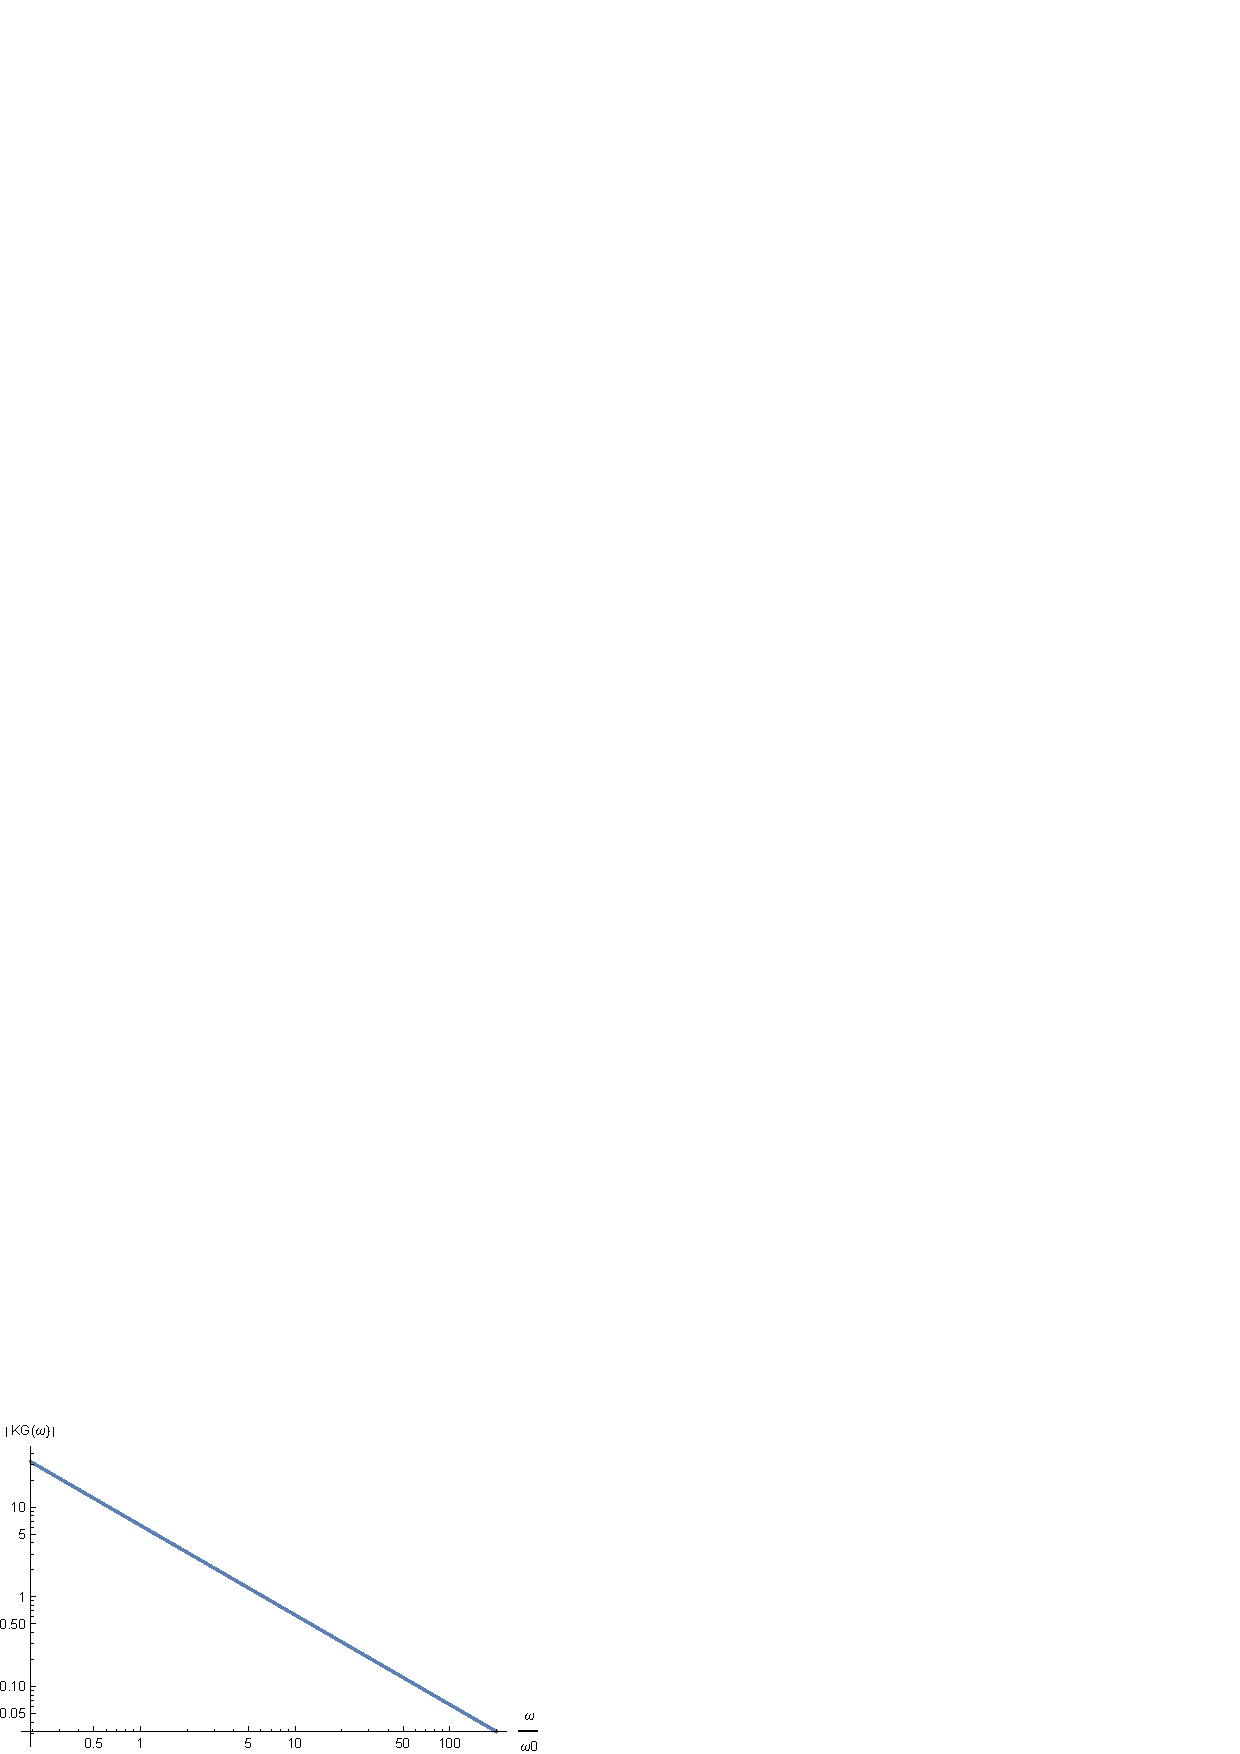
\includegraphics[width=0.45\textwidth]{bode_3}
	\quad
	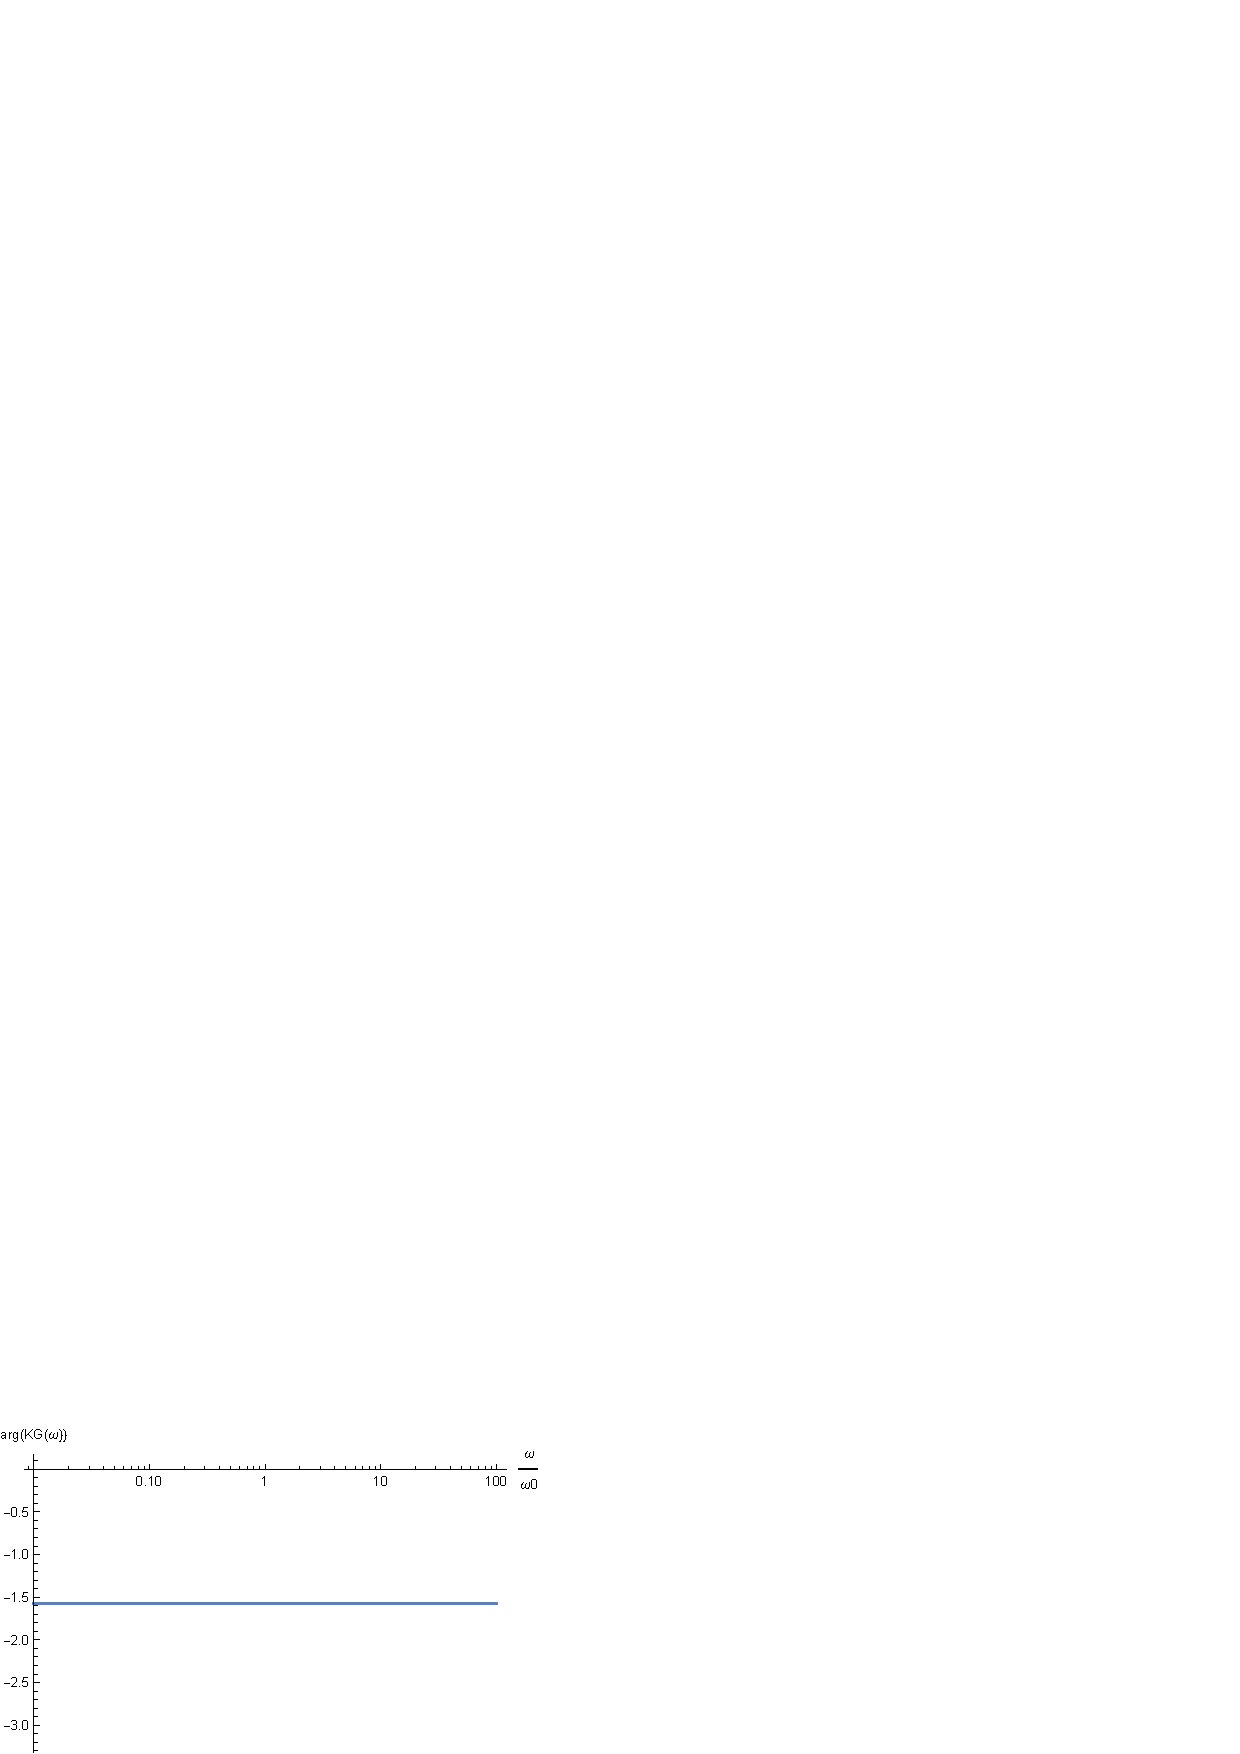
\includegraphics[width=0.45\textwidth]{bode_4}
	\caption{Open-loop gain $KG$ for oscillator-PID system with natural resonance frequency $\omega_0$ ``tweaked away.'' The phase lag is constantly $\pi/2$ and the gain decreases like $1/\omega$ Again, $\beta = 2,\omega_0 = 2\pi$.} %
	\label{fig:bode_2}
\end{figure}






\subsection{The P-gain}

Suppose we set $K_i = K_d = 0$ and only have $K_p$. Is $K_p$ enough to bring the system to $r(t)$? The answer is ``Yes, but not very well.'' Here's why. In time domain, the ODE is 
\begin{equation*}
\ddot{x}(t) + \beta \dot{x} + \omega_0^2 x(t) = \omega_0^2 K_p (r(t) - x(t)). 
\end{equation*} 
Rearranging gives
\begin{equation*}
\ddot{x}(t) + \beta \dot{x} + \omega_0^2 (1+K_p) x(t) = \omega_0^2 K_p P r(t). 
\end{equation*}
This is basically a driven harmonic oscillator with a modified natural frequency of $\omega_P = \omega_0 \sqrt{1+K_p}$. When the proportional gain $K_p$ is very high $(K_p \gg 1)$, the modified natural frequency is much greater than the original natural frequency, $\omega_P \gg \omega$. As a result, the oscillator can follow the reference without significant phase lags even with $\omega$'s much larger than $\omega_0$. Meanwhile, the gain can be calculated from  
\begin{equation*}
x(\omega\ll \omega_P) \approx \f{K_p}{1+K_p} r(\omega) \approx r(\omega),
\end{equation*}
which says that the gain is very close to unity $\omega$ within $\omega_P$ (again, assuming that $P\gg 1$). Both of these features can be seen in Figure \ref{fig:bode_3}. 


\begin{figure}
	\centering
	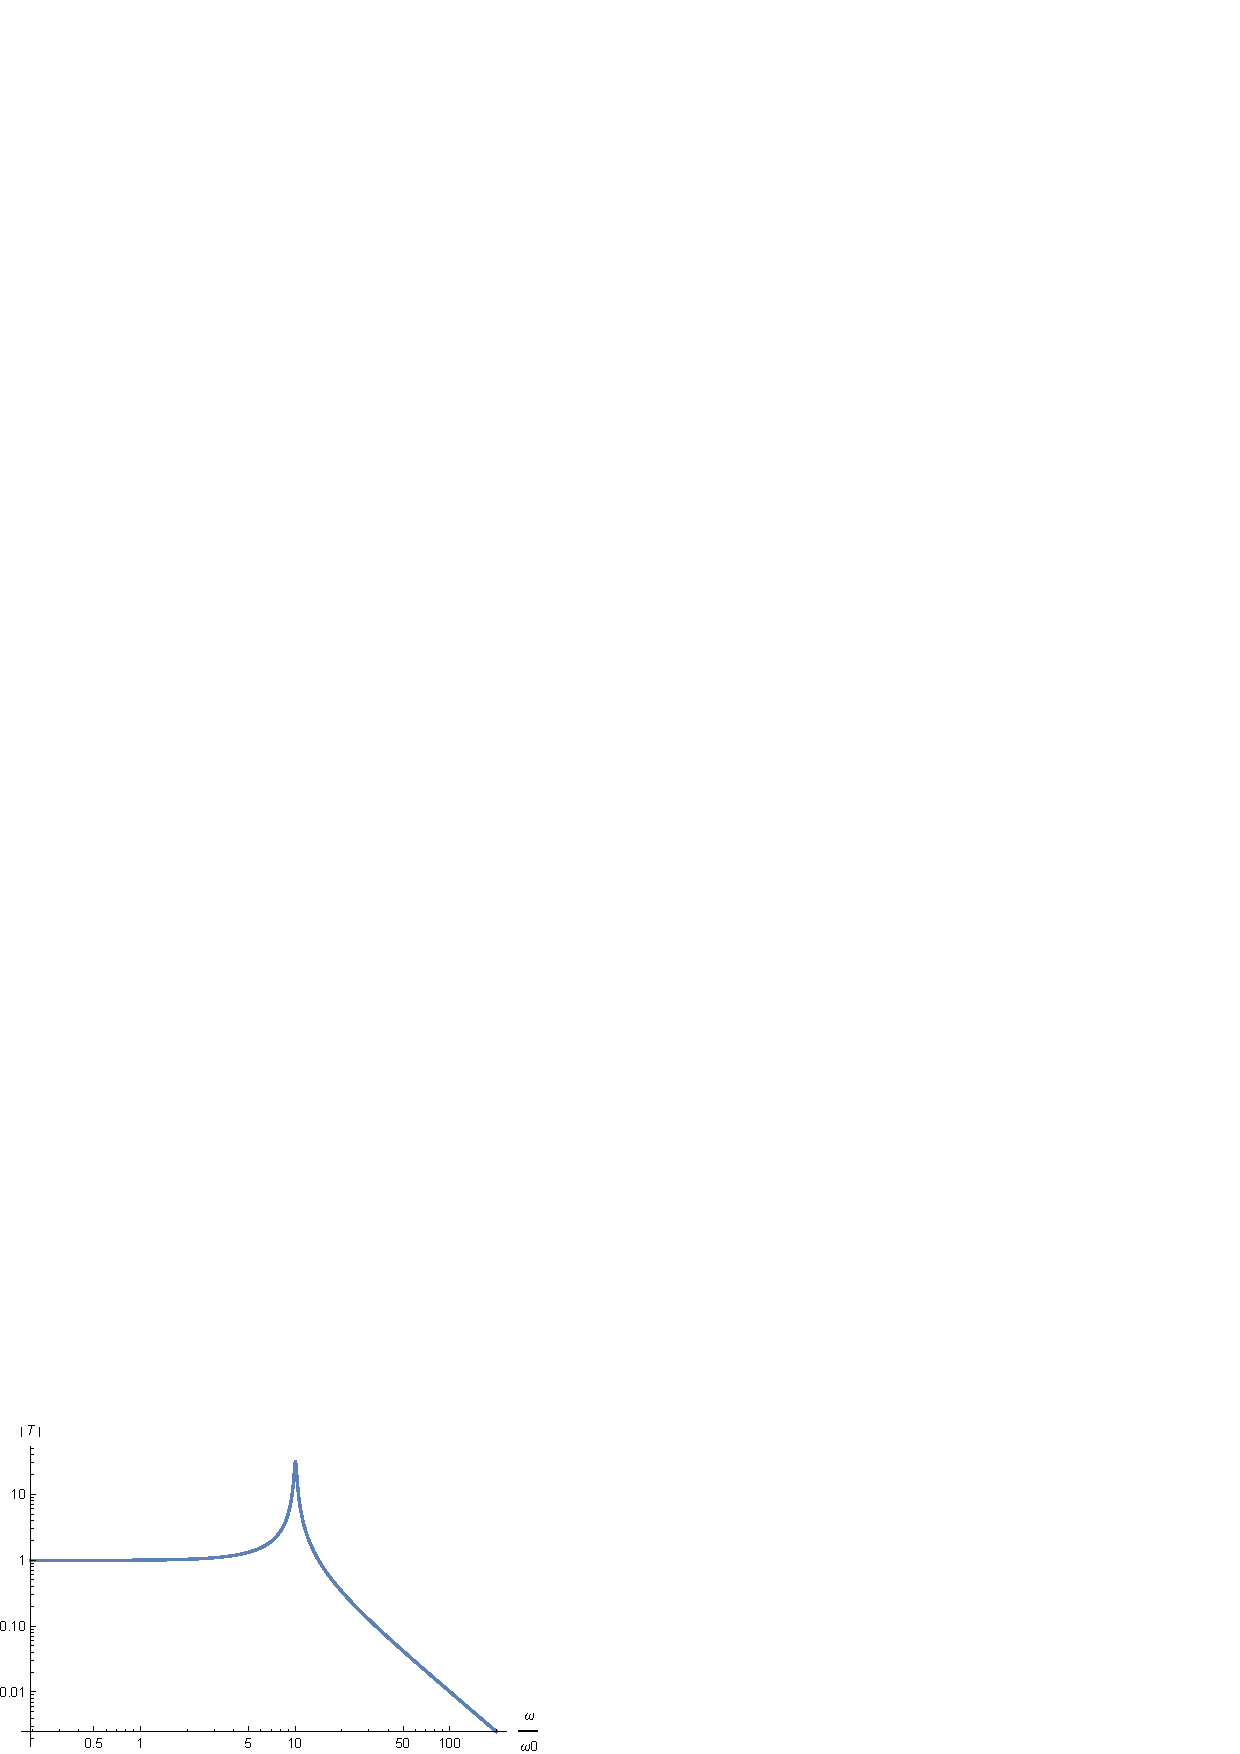
\includegraphics[width=0.45\textwidth]{bode_5}
	\quad
	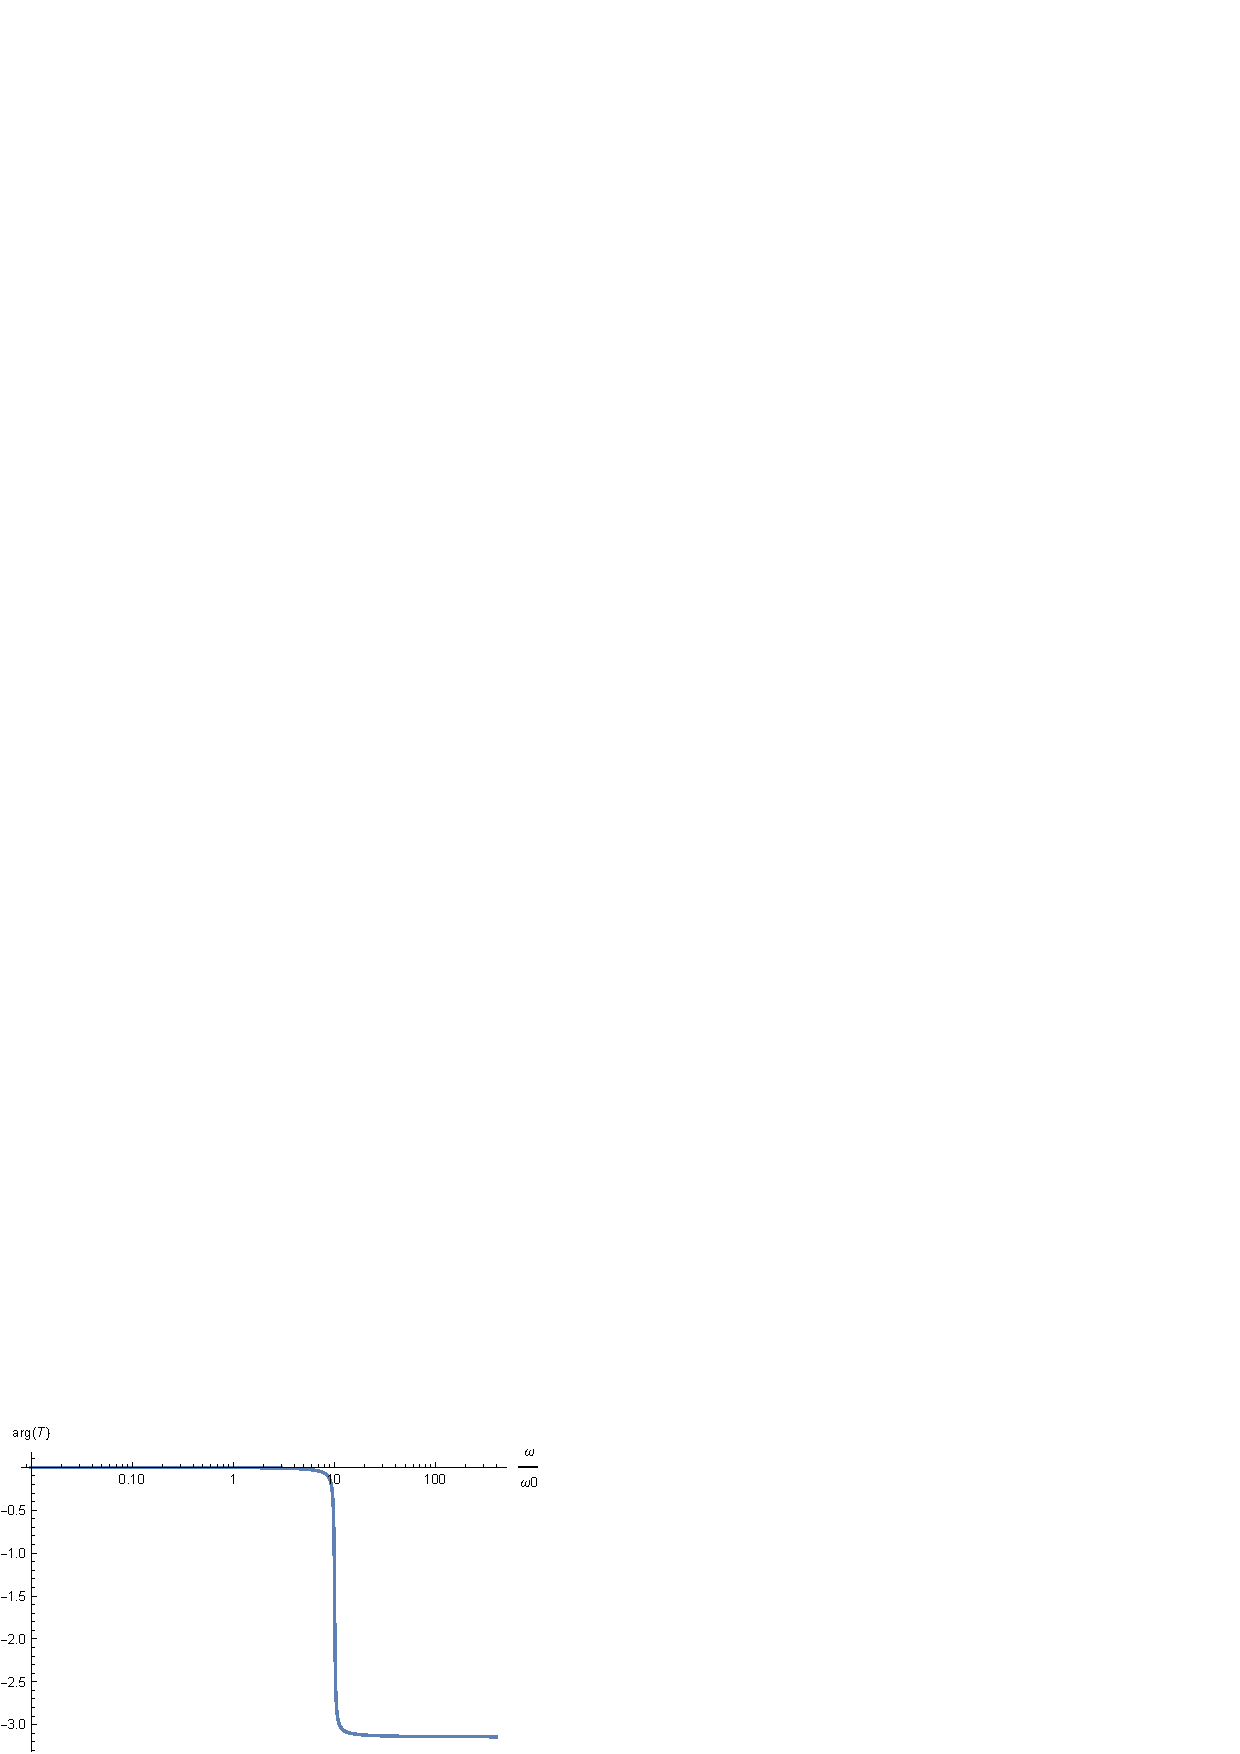
\includegraphics[width=0.45\textwidth]{bode_6}
	\caption{Bode plot for $P$-controller. Here, $\beta = 2,\omega_0 = 2\pi$, and $K_p = 100$.} %
	\label{fig:bode_3}
\end{figure}



So why not use only P rather than PID? Well, the catch is that we just pushed the resonance frequency of our system to a much higher value which could be comparable to variations due to noise. If noise is around the modified resonance frequency $\omega_P$ then resonance will kick in. There are two types of noise: $d(t)$ due to disturbance to our system (more or less ``mechanical'') and $\xi(t)$ which is measurement noise (usually fast). The total dynamics will then be 
\begin{equation*}
x(\omega) = K(\omega)G(\omega) \epsilon(\omega) + d(\omega)
\end{equation*}
where 
\begin{equation*}
\epsilon(\omega) = r(\omega) - x(\omega) - \xi(\omega)
\end{equation*}
which gives
\begin{equation*}
x(\omega) = \f{K(\omega)G(\omega)}{1+K(\omega)G(\omega)}[r(\omega)-\xi(\omega)] + \f{1}{1+K(\omega)G(\omega)}d(\omega).
\end{equation*}
From here, we see that for really high proportional gain (i.e., $\abs{K} \gg 1$), the $d(\omega)$ noise will be suppressed up to $\omega_P$, which is good. However, the measurement noise $\xi(t)$ gets mixed up with the referent signal $r(\omega)$ and amplified. One can define the tracking error, which is the difference between the reference $r$ and the actual position $x$ (all error free), in terms of the errors:
\begin{equation*}
\epsilon_0 \equiv r - x = S(r-d) + T\xi
\end{equation*}
with the \textbf{sensitivity function} $S$ and \textbf{complimentary sensitivity function} $T$. The goal is to make $\epsilon_0$ as small as possible, but we're limited by the fact that $S+T=1$ for all $\omega$. For small $S$ disturbances are rejected but then $T$ is large and measurement noise is coupled in, and vice versa.
For more information on this part, the reader may reference \cite{bechhoefer2005feedback}.


\subsection{The I-gain}



\subsection{Instability}

\subsection{The D-gain}




\section{Experimentally tuning P-I-D with MATLAB}



\subsection{MATLAB code}

\begin{lstlisting}
% Author: Huan Q. Bui
% June 30, 2021
% Simple demo of PID control 
% for a driven damped HO

% Inspired by: https://robotics.stackexchange.com...
% /questions/6859/how-to-implement-tracking-problem-with-pid-controller


clear all; close all; clc;

global error r dt time_array;

error = 0;
dt = 0.1;
stoptime = 100;

%%% create set(point)function
r = ones(stoptime/dt,1); % setpoint
%r(1:10) = 0;
r(floor((stoptime/dt)/4):(stoptime/dt)/2) = 0;
r(floor(3*(stoptime/dt)/(4)):end) = 0;
% define time array so that dimension matches setpoint r(t)
time_array = 0:dt:dt*(numel(r)-1);


x0 = [0; 0]; % initial condition, position & velocity = 0;
options = odeset('Reltol',dt,'Stats','off');
tspan = [time_array(1),time_array(end)];
[t_ode, x] = ode45(@ODESolver, tspan, x0, options);


% interpolate setpoint function 
% so that we have r(t) with the same dimension as 
% x(t) from ODE (which has finer resolution)
r_desired_ode = interp1(time_array,r,t_ode);
err = x(:,1) - r_desired_ode; % Error signal


%%% plotting %%%

figure(1)
plot(t_ode,x(:,1))
hold on 
plot(t_ode,r_desired_ode)
xlabel('Time (sec)');
ylabel('Position', 'Interpreter','LaTex');
legend('Actual position', 'Desired position')
grid on
hold off


% figure(2)
% plot(t_ode, x(:,2), 'r', 'LineWidth', 2);
% title('Velocity','Interpreter','LaTex');
% xlabel('time (sec)');
% ylabel('$\dot{\theta}(t)$', 'Interpreter','LaTex');
% grid on

%%% %%%

function dxdt = ODESolver(t, x)

persistent r_old t_old;
global error r time_array;

if isempty(r_old)
r_old = 0;
t_old = 0;
end

% Parameters:
beta = 1;
omega0 = 2*pi;

% PID tuning
Kp = 100;
Ki = 20;
Kd = 7;

% dr/dt: find the derivative of r(t) for D-gain:
r_now = interp1(time_array,r,t);
if t == t_old
drdt = 0;
else
drdt  = (r_now - r_old)/(t-t_old);
end
r_old = r_now;

% u: control function
u = Kp*(r_now - x(1))... % P-gain
+ Kd*(drdt - x(2))... % D-gain
+ Ki*error; % I-gain;

% new error signal, obtained by accumulating errors (integral)
error = error + (r_now - x(1))*(t-t_old);

% 2x2 system of 1st-order ODEs
% initialize: matrix with position & velocity
dxdt = zeros(2,1);
dxdt(1) = x(2); % velocity
dxdt(2) = (omega0^2)*u - beta*x(2) - (omega0^2)*x(1); % acceleration

t_old = t;
end
\end{lstlisting}




\nocite{bechhoefer2005feedback}
\nocite{zwierleinPID}



\bibliography{BUI_PID} 
\bibliographystyle{ieeetr}









\end{document}